\documentclass[a4paper]{article}

%% Language and font encodings
\usepackage[english]{babel}
\usepackage[utf8x]{inputenc}
\usepackage[T1]{fontenc}

%% Sets page size and margins
\usepackage[a4paper,top=3cm,bottom=2cm,left=3cm,right=3cm,marginparwidth=1.75cm]{geometry}

%% Useful packages
\usepackage{amsmath}
\usepackage{graphicx}
\usepackage[colorinlistoftodos]{todonotes}
\usepackage[colorlinks=true, allcolors=blue]{hyperref}
\title{Navier Stokes Equations}
\author{Quanhui Zhu}

\begin{document}
\maketitle

\begin{abstract}
  This project discusses how to solve Navier-Stokes equations by mixed
  element methods. It begins with the Stokes equations solver, and
  also its AMG block precondition skills; then a Newton iteration is
  designed to deal the nonlinear discretized system of Navier-Stokes
  equations.  For large viscosity parameter ($\geq 0.02$, or RE$\leq
  50$), the solutions of steady Navier-Stokes equations can be solved
  directly by using an ILU preconditioner, while for the large
  viscosity ($\geq 0.0005$, or RE$\leq 2000$) cases, a time dependent
  Navier-Stokes solver is implemented to approximate the steady
  solution by making the computing time sufficient large. A series
  bentchmark simulations are fulfiled to check the correctness of the
  algorithms and codes.
\end{abstract}


\section{Stokes Equations}

\subsection{Weak Form}

The Stokes equations we discussed take the form as
\begin{equation}
\begin{array}{rcl}
-\nabla^2 \vec{u} + \nabla p &=& \vec{0} \\
\nabla \cdot \vec{u} &=& \vec{0}
\label{eq::Stokes-problem}
\end{array}
\end{equation}
The equations (\ref{eq::Stokes-problem}) are the fundamental model of
viscous flow with boundary values considered that
\begin{equation}
\vec{u} = \vec{w} \ on \ \partial \Omega_D ,\quad \frac{\partial
  \vec{u}}{\partial n} - \vec{n} p = \vec{s} \ on \ \partial \Omega_N.
\end{equation}
Here the variable $p$ is the pressure.

We use the P2-P1 mixed elements, or famous as Taylor-Hood elements
\cite{Lee2005Finite} to discrete the equations. And the weak form of
the equations (\ref{eq::Stokes-problem}) reads
\begin{equation}
\begin{array}{rcl}
-\int_\Omega \nabla^2 \vec{u} \cdot \vec{v} + \nabla p &=& 0\\
\int_\Omega q\nabla \cdot \vec{u} &=&0
\label{eq::Stokes-weakform}
\end{array}
\end{equation}

It can be reformed by applying Green Theorem as
\begin{equation}
\begin{array}{rcl}
\int_\Omega \nabla \vec{u} : \nabla \vec{v} - \int_\Omega p\nabla
\cdot \vec{v} &=& \int_{\partial \Omega_N}\vec{s}\cdot \vec{v} \quad
for \ all \ \vec{v} \in H^1_{E_0}\\ \int_\Omega q\nabla \cdot \vec{u}
&=& 0 \quad for \ all \ q\in L_2(\Omega)
\label{eq::Stokes}
\end{array}
\end{equation}

Assume that the basis functions of the velocity space are
{$\vec{\phi}_j$} such that
\begin{equation}
\vec{u}_h = \sum^{n_u}_{j=1}u_j\vec{\phi}_j + \sum^{n_u + n_\partial}_{j=n_u+1}u_j\vec{\phi}_j,
\label{eq::Stokes-u}
\end{equation}
while the basis functions of the pressure space are $\psi_k$ such that
\begin{equation}
p_h = \sum^{n_p}_{k=1}p_k\psi_k,
\label{eq::Stokes-p}
\end{equation}
then the weak form can be expressed by the following linear system:
\begin{equation}
\left[ \begin{array}{ccc}
A & B^T \\
B & 0
\end{array}
\right]
\left[\begin{array}{ccc}
u\\
p
\end{array}
\right]=
\left[\begin{array}{ccc}
f\\
g
\end{array}
\right]
\label{mt::Stokes}
\end{equation}
Here the matrix $A$ and $B$ are given by
\begin{equation}
\begin{array}{rcl}
A &=& [a_{ij}], \quad a_{ij} = \int_{\Omega} \nabla \vec{\phi}_i :
\nabla \vec{\phi}_j,\\ B &=& [b_{kj}], \quad b_{kj} = -\int_{\Omega}
\psi_k\nabla \cdot \vec{\phi_j},
\end{array}
\end{equation}
respectively.


\subsection{Matrix Form}

Specially, we set the \{$\vec{\phi}_i$\} a standard basis functions that
\begin{equation}
\{\vec{\phi_1},\vec{\phi_2},\cdots,\vec{\phi_{2n}} \}:=\{(\phi_1,0)^T,\cdots,(\phi_n,0)^T,(0,\phi_1)^T,\cdots,(0,\phi_n)^T\}
\label{eq::basisfunction}
\end{equation}
With $u:=([u_x]_1,\cdots,[u_x]_n,[u_y]_1,\cdots,[u_y]_n)$, system (\ref{mt::Stokes}) can be rewritten as
\begin{equation}
\left[ \begin{array}{ccc}
A & 0 & B_x^T \\
0 & A & B_y^T \\
B_x & B_y & 0
\end{array}
\right]
\left[\begin{array}{ccc}
u_x\\
u_y\\
p
\end{array}
\right]=
\left[\begin{array}{ccc}
f_x\\
f_y\\
g
\end{array}
\right]
\label{Stokes}
\end{equation}
where the $n\times n$ matrix $A$ is the scalar Laplacian matrix, and the $n_p\times n$ matrices $B_x$ and $B_y$ represent weak derivatives in the $x$ and $y$ direction that 	
\begin{equation}
\begin{array}{rcl}
A &=& [a_{ij}], \quad a_{ij} = \int_{\Omega} \nabla \phi_i : \nabla \phi_j \\
B_x &=& [b_{x,ki}], \quad b_{x,ki} = -\int_{\Omega} \psi_k \frac{\partial \phi_i}{\partial x} \\
B_y &=& [b_{y,kj}], \quad b_{y,kj} = -\int_{\Omega} \psi_k \frac{\partial \phi_j}{\partial y} \\
\end{array}
\label{Stokes-mtvalue}
\end{equation}
 \\
\subsection{Precondition}
The basis functions given by mixed finite element methods are piecewise linear. We have the matrix system symmetric positive definite and highly sparse. Thus proper precondition is needed to improve computing efficiency. There is a AMG block preconditioner for the Stokes matrix.
\begin{equation}
M = \left[ \begin{array}{ccc}
A & 0 & 0 \\
0 & A & 0 \\
0 & 0 & Q
\end{array}
\right]
\end{equation}
where $Q$ is a $n_p\times n_p$ pressure quality matrix.
\begin{equation}
Q = [q_{ij}], \quad q_{ij} = \int_{\Omega} \psi_i\psi_j
\label{pr::Q}
\end{equation}
Specially, as we just need a preconditioner and Q is a diagonally dominant matrix, we can set Q a diagonal matrix. It makes the matrix easier but has a similar effect.
\subsection{Result}
We consider the question given that: $\Omega = [0,1]\times[0,1]$, the boundary value
\begin{equation}
\left\lbrace
\begin{array}{rcl}
u_x &=& 1,\quad on \ \{(x,y): x \in [0,1] \ and \ y = 1\}\\
u &=& 0,\quad others
\end{array}
\right.
\label{bd::value1}
\end{equation}
The mesh relies on easymesh and the finite element methods rely on AFEPack and dealII 8.1.0. We set $h=0.05$ to see a brief solution of Stokes equations.

\begin{figure}[h]
\centering
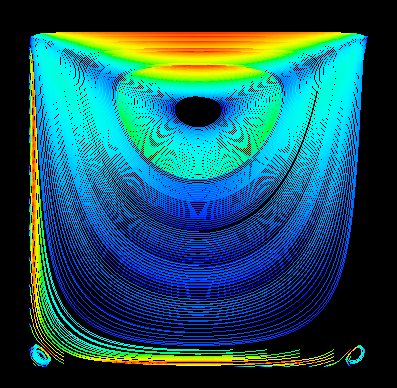
\includegraphics[scale = 0.4]{images/Stokes.png}
\caption{Stokes Solution}
\label{im::Stokes-Solution}
\end{figure}

From the Figure \ref{im::Stokes-Solution}, the Stokes system is symmetric and stable. There are two counter-rotating recirculations(called Moffatt eddies). The figure gives us a brief understanding of fluid system.


\section{Navier Stokes}
\subsection{Weak Form}
Let's consider the Navier-Stokes equations now:
\begin{equation}
\begin{array}{rcl}
-\nu \nabla^2 \vec{u} + \vec{u}\cdot \nabla \vec{u} + \nabla p &=& \vec{F} \\
\nabla \cdot \vec{u} &=& \vec{0}
\label{eq::Navier-Stokes-problem}
\end{array}
\end{equation}
As we did before, a standard weak form is given that
\begin{equation}
\begin{array}{rcl}
-\nu\int_\Omega \nabla^2 \vec{u} \cdot \vec{v}+\int_{\Omega}\vec{u}\cdot\nabla\vec{u}\cdot\vec{v} + \nabla p &=& \int_{\Omega}\vec{F}\cdot \vec{v},\quad for \ all \ \vec{v} \in H^1_{E_0} \\
\int_\Omega q\nabla \cdot \vec{u} &=&0,\quad for \ all \ q \in L_2(\Omega)
\label{eq::Navier-Stokes-weakform}
\end{array}
\end{equation}
The problem can't be solved directly because of the nonlinear item $\vec{u}\cdot \nabla \vec{u}$. We consider a newton iteration that $x_{n+1}=x_{n} - (A(x_n)-b)\cdot J(A(x_{n}))^{-1}$. $J(A)$ means $A$'s Jacobi matrix. The iteration form is that
$$ J(A(x_n))\Delta x = b - A(x_n)$$
\indent Having same basis functions as (\ref{eq::basisfunction}), a similar matrix system shows that
\begin{equation}
\left[ \begin{array}{ccc}
A + N +W_{xx} & W_{xy} & B_x^T \\
W_{yx} & A +N +W{yy}& B_y^T \\
B_x & B_y & 0
\end{array}
\right]
\left[\begin{array}{ccc}
\Delta u_x\\
\Delta u_y\\
\Delta p
\end{array}
\right]=
\left[\begin{array}{ccc}
f_x\\
f_y\\
g
\end{array}
\right]
\label{Navier-Stokes}
\end{equation}
Where $A$ and $B$ are same as before and the matrix $N$ is the $n\times n$ scalar convection matrix
\begin{equation}
N = [n_{ij}], \quad n_{ij} = \int_{\Omega} (\vec{u}_h\cdot \nabla\phi_j)\phi_i
\label{mt::N}
\end{equation}
The $n\times n$ matrices $W_{xx}, W_{xy}, W_{yx}, W_{yy}$ represent weak derivatives of the current velocity in the $x$ and $y$ directions
\begin{equation}
W_{xy} = [w_{xy,ij}],\quad w_{xy,ij} = \int_{\Omega} \frac{\partial u_x}{\partial y}\phi_u \phi_j
\label{mt::W}
\end{equation}
In the iteration, the right item is the residual
\begin{equation}
f = [f_i],\quad f_i=\int_{\Omega}(\vec{F}\cdot\vec{\phi}_i-\vec{u}_h\cdot\nabla\vec{u}_h\cdot\vec{\phi}_i-\nu\nabla\vec{u}_h:\nabla\vec{\phi}_i+p_h(\nabla\cdot\vec{\phi}_i))
\end{equation}
\begin{equation}
g = [g_k],\quad g_k=\int_{\Omega}\psi_k(\nabla \cdot \vec{u}_h)
\end{equation}
When we calculate $f$ in $x$ and $y$ directions, it changes that
\begin{equation}
\begin{array}{rcl}
f_x &=& [f_{xi}],\quad f_{xi}=\int_{\Omega}(F_x\cdot\phi_i-\vec{u}_h\cdot\nabla u_x\cdot\phi_i-\nu\nabla u_x:\nabla\phi_i+p_h(\nabla\cdot\phi_i)) \\
f_y &=& [f_{yi}],\quad f_{yi}=\int_{\Omega}(F_y\cdot\phi_i-\vec{u}_h\cdot\nabla u_y\cdot\phi_i-\nu\nabla u_y:\nabla\phi_i+p_h(\nabla\cdot\phi_i))
\label{mt::f}
\end{array}
\end{equation}
\subsection{Result}
First we consider one problem which has an accurate solution that
\begin{equation}
u_x = 1-y^2;\quad u_y = 0;\quad p=-2\nu x;
\label{pr::accurate}
\end{equation}

It's called Poiseuille channel flow. The square domain $\Omega = (-1,1)^2$. We set mesh $h=0.2,\ 0.1,\ 0.05,\ 0.02$ and $\nu=1$, then plot the image about numerical error $||u_h-u_0||_2$ and $h$.
\begin{figure}[h]
\centering
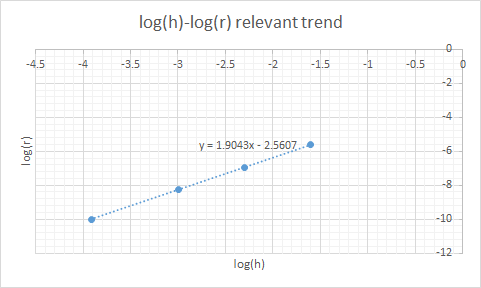
\includegraphics[scale = 0.8]{images/convergence.png}
\caption{the relevance between log(h) and log(r)}
\label{im::log(h)-res}
\end{figure}
\\
The slope of the figure (\ref{im::log(h)-res}) is 1.9043. We can see the method converges with a about $O(h^2)$ order. \\




\indent Then under same boundary value as (\ref{bd::value1}), let's see what difference will appear between Navier-Stokes fluid and Stokes fluid when $\nu=1,\ 0.1,\ 0.01,\ h=0.05$. (We use ilu precondition here provided by dealII)
\begin{figure}[h]
\centering
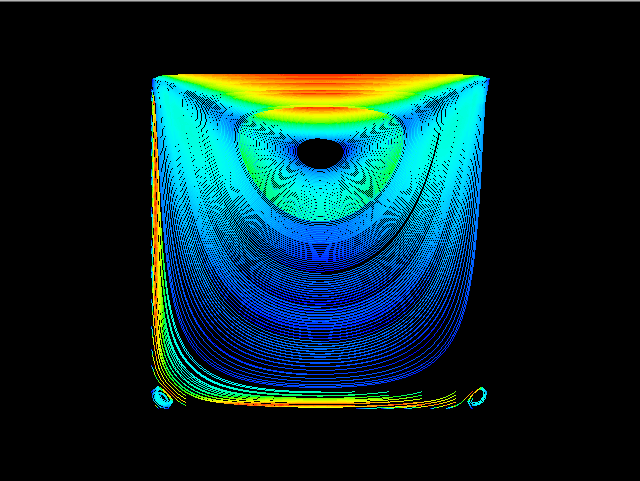
\includegraphics[scale = 0.2]{images/a.png}
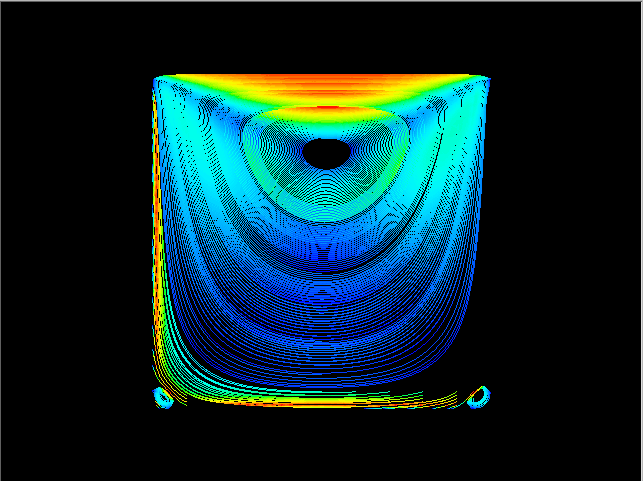
\includegraphics[scale = 0.2]{images/b.png}
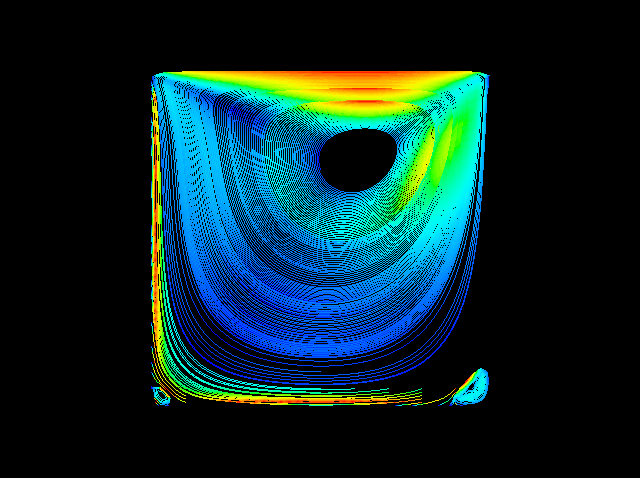
\includegraphics[scale = 0.2]{images/c.png}
\caption{the Navier-Stokes Solution($\nu$=1, 0.1, 0.01)}
\label{im::Navier-Stoke-solution}
\end{figure}
\\
We can see that the fluid is not symmetric again. With the viscosity growing, the Moffatt eddies become more unstable. The right side corner eddy catches more energy from the prime eddy. We continue calculating until the viscosity comes to 0.0001. If the viscosity becomes smaller, the process even don't converge. New methods is needed now.
\subsection{Time Depending}
We consider the equations that
\begin{equation}
\begin{array}{rcl}
\frac{\partial\vec{u}}{\partial t}-\nu \nabla^2 \vec{u} + \vec{u}\cdot \nabla \vec{u} + \nabla p &=& \vec{F} \\
\nabla \cdot \vec{u} &=& \vec{0}
\label{eq::Timedepending-problem}
\end{array}
\end{equation}
We add a time-control item to Navier-Stokes equations. When it converges, the solution is the same as Navier-Stokes under same boundary value.


We use implicit format that $\frac{\partial u}{\partial t} = \frac{u^{n+1}-u^{n}}{\Delta t}$ in $x$ and $y$ directions.
The iteration becomes that
\begin{equation}
\left[ \begin{array}{ccc}
A + N +W_{xx} + T_x & W_{xy} & B_x^T \\
W_{yx} & A +N +W{yy} + T_y& B_y^T \\
B_x & B_y & 0
\end{array}
\right]
\left[\begin{array}{ccc}
\Delta u_x\\
\Delta u_y\\
\Delta p
\end{array}
\right]=
\left[\begin{array}{ccc}
f_x + t_x\\
f_y + t_y\\
g
\end{array}
\right]
\label{Timedepending}
\end{equation}
The $T$ is the $n\times n$ time developing matrix
\begin{equation}
T = [t_{ij}],\quad t_{ij}=\frac{1}{\Delta t}\int_{\Omega}\vec{\phi}_i\cdot\vec{\phi}_j
\end{equation}
and the vector $t$ is the former velocity value
\begin{equation}
t = [t_{k}],\quad t_{k}=\frac{1}{\Delta t}\int_{\Omega}\vec{u}_h\cdot\vec{\phi}_i
\end{equation}
\\


Now let's try to solve the Navier-Stokes equations while $\nu=0.00005(Re=2000)$. The solution is that
\begin{figure}[h]
\centering
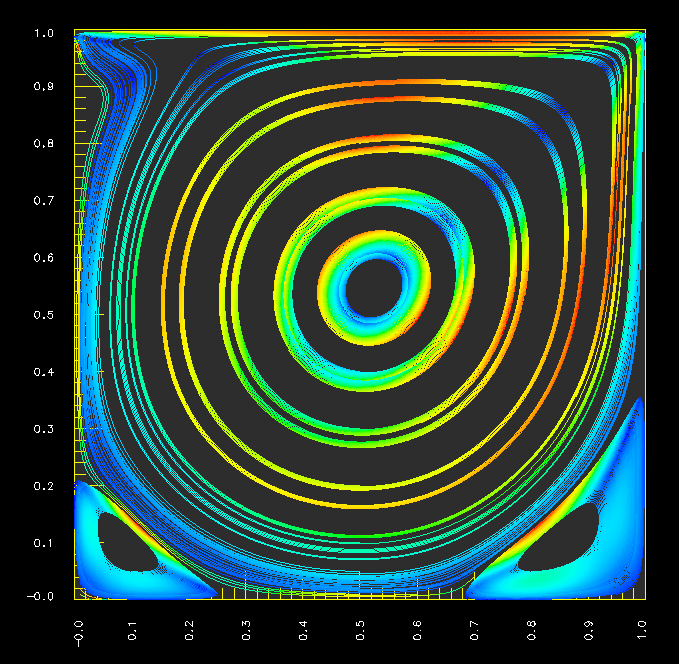
\includegraphics[scale = 0.5]{images/e.png}
\caption{the Navier-Stokes fluid while $\nu=0.00005$}
\label{im::d}
\end{figure}


In the figure (\ref{im::d}), new eddy comes to appear and the fluid becomes unstable. When the Re($\frac{1}{\nu}$) grows again, the model can't explain the phenomenon any more. It needs to introduce more theories.
\section{Future Work}
\subsection{3D}
Actually we just calculate the problem in the plane. For practical calculating, we should extend it to 3D space. It doesn't exist essential difficulty. We just change the matrix (\ref{Navier-Stokes}) that
\begin{equation}
\left[ \begin{array}{cccc}
A + N +W_{xx} & W_{xy} & W_{xz} & B_x^T \\
W_{yx} & A +N +W{yy}& W_{yz} & B_y^T \\
W_{zx} & W_{zy}  &A + N + W_{zz} & B_z^T \\
B_x & B_y &B_z& 0
\end{array}
\right]
\left[\begin{array}{cccc}
\Delta u_x\\
\Delta u_y\\
\Delta u_z\\
\Delta p
\end{array}
\right]=
\left[\begin{array}{cccc}
f_x\\
f_y\\
f_z\\
g
\end{array}
\right]
\label{3D-Navier-Stokes}
\end{equation}
The difficulty is we use easymesh to build the 2D mesh. New 3D mesh-building tools is required now.
\subsection{Precondition}
With the matrix size growing, better precondition is needed. Otherwise we can hardly solve the linear equations. Considering the time-depending Navier-Stokes equations (\ref{eq::Timedepending-problem}), we use semi-implicit scheme that
\begin{equation}
\begin{array}{rcl}
\frac{\vec{u}^{n+1}-\vec{u}^n}{\Delta t} - \nu \nabla^2 \vec{u}^{n+1} + \vec{u}^{n}\cdot \nabla \vec{u}^n + \nabla p^{n+1} &=& \vec{F} \\
\nabla \cdot \vec{u}^{n+1} &=& \vec{0}
\label{eq::implicit and explicit}
\end{array}
\end{equation}
Thus we change the equations to a time-developinig Stokes equations. Now we can use proper precondition like AMG block precondition given before to make the calculating faster.

\bibliographystyle{alpha}
\bibliography{sample}

\end{document}
